\subsection{GUI}

FLOps uses MLFlow's GUI and does not modify it.
Therefore, this chapter only provides a brief selection of impressions of the GUI.
Excellent further details are available directly at MLflow \cite{mlflow:homepage}.

\begin{figure}[p]
    \begin{adjustwidth}{-0.1\paperwidth}{-0.1\paperwidth}
        \centering
        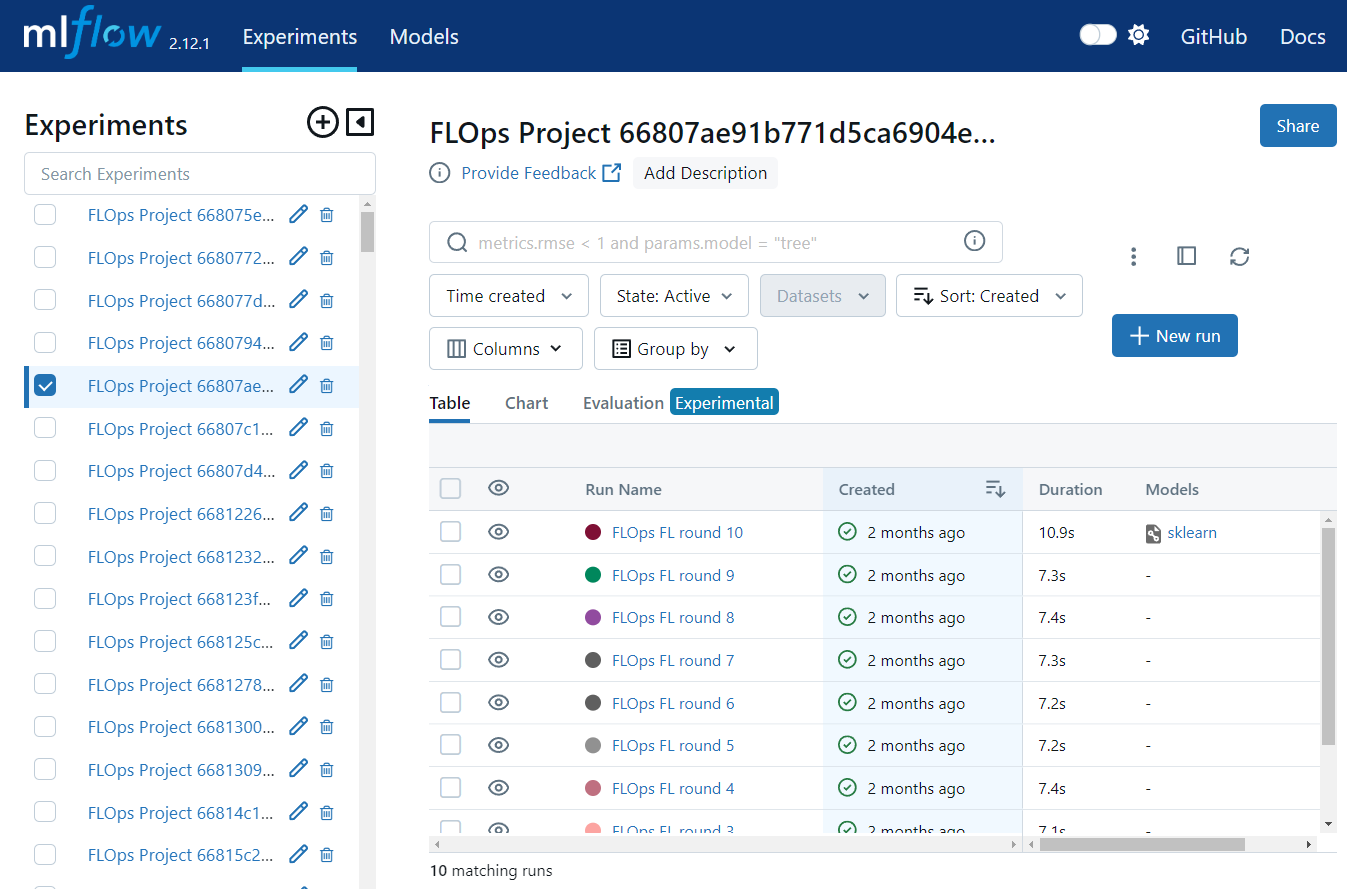
\includegraphics[width=0.90\paperwidth]{gui_ss_1.png}
        \caption{MLflow's GUI Screenshot - Experiments Overview}
        \label{fig:gui_ss_1}
    \end{adjustwidth}
\end{figure}

The first screenshot \ref{fig:gui_ss_1} shows MLflow's experiments overview page.
The left column lists all recorded experiments/projects.
Only a single one is currently selected.
Details about it are displayed to the right.
Multiple experiments can be selected simultaneously to view their combined contents.
The centerpiece offers a table view of the different FL rounds.
Users can customize and sort this table to their liking.
Each table row depicts a single FL round, when it was recorded, and its duration.
Only the best round contains a logged model.
In this example, the best round was the last (10th) round.

\begin{figure}[p]
    \begin{adjustwidth}{-0.1\paperwidth}{-0.1\paperwidth}
        \centering
        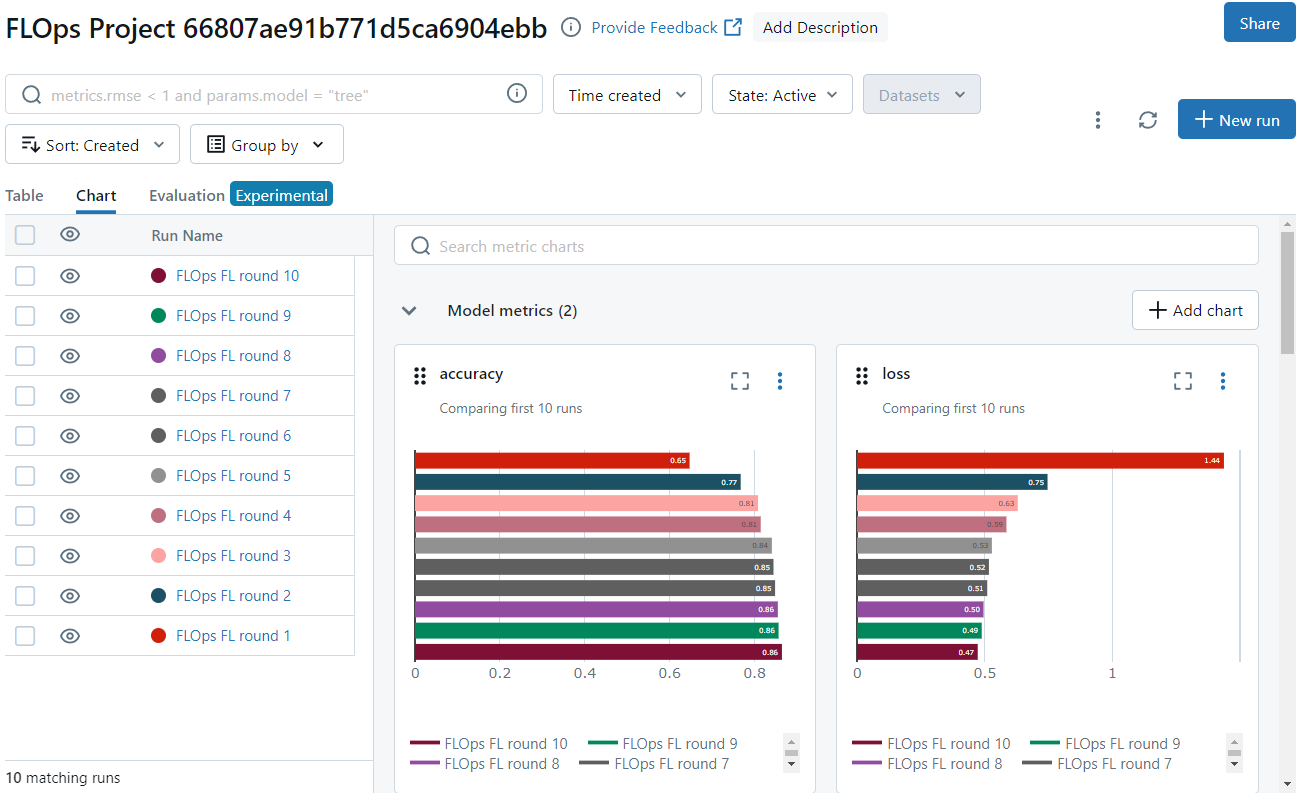
\includegraphics[width=0.90\paperwidth]{gui_ss_2.png}
        \caption{MLflow's GUI Screenshot - Experiment Details}
        \label{fig:gui_ss_2}
    \end{adjustwidth}
\end{figure}

Figure \ref{fig:gui_ss_2} shows the detailed view of a single recorded experiment/project.
Currently, FLOps focuses on the model's accuracy and loss.
The centerpiece of the screenshot shows the evolution of both across different FL rounds.
It shows that the model's accuracy improved, and its loss decreased over time.
FLOps users can access this GUI during FL training and observe how this FL-rounds table grows in real-time.

\begin{figure}[p]
    \centering
    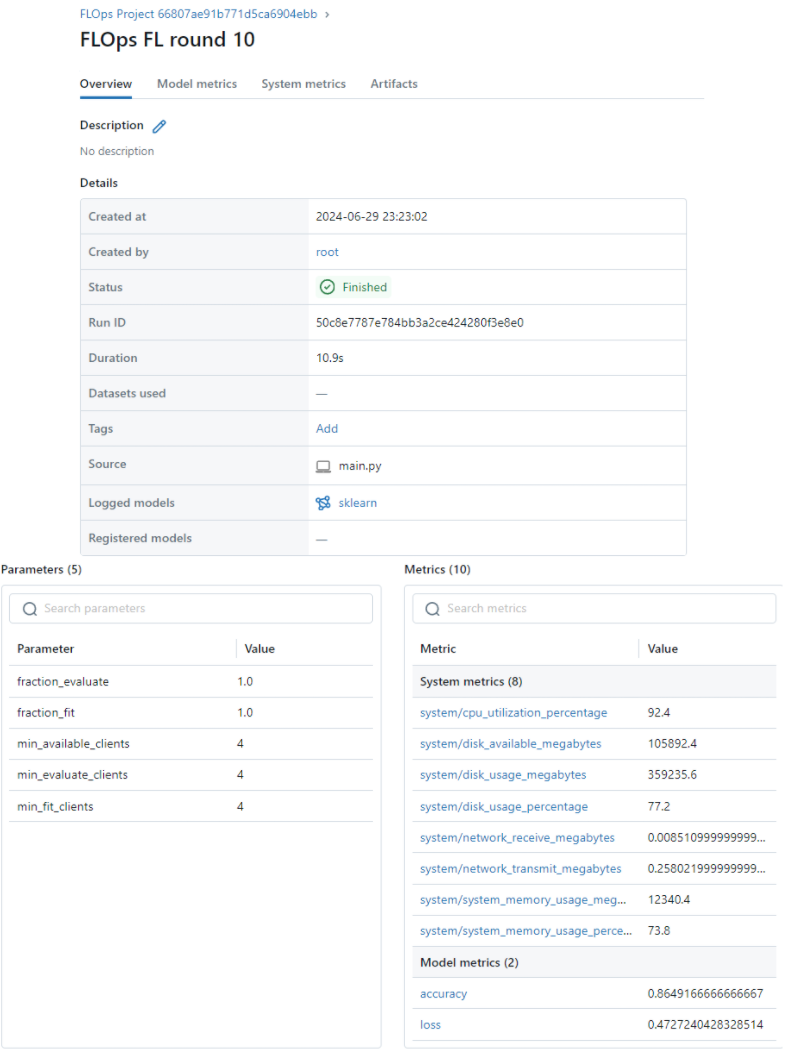
\includegraphics[height=1.0\textheight]{gui_ss_3.png}
    \caption{MLflow's GUI Screenshot - FL Round Details}
    \label{fig:gui_ss_3}
\end{figure}

The third screenshot \ref{fig:gui_ss_3} depicts concrete FL round details.
These details include general information such as if and what model was recorded, the run/round ID, or when the run was created.
In addition, it displays custom parameters that FLOps injected, including the user-provided number of clients/learners via the SLA.
This page also displays other metrics, such as accuracy or system metrics.

\begin{figure}[p]
    \begin{adjustwidth}{-0.1\paperwidth}{-0.1\paperwidth}
        \centering
        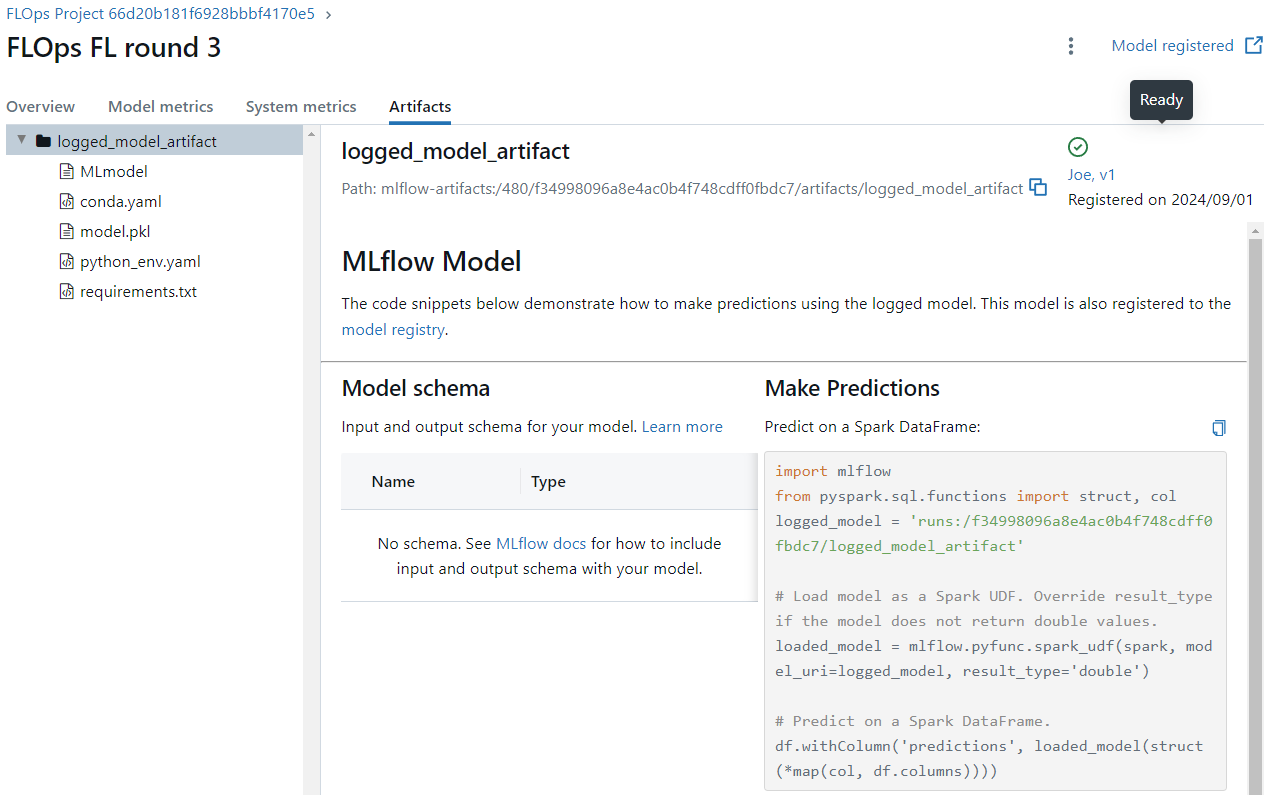
\includegraphics[width=0.90\paperwidth]{gui_ss_4.png}
        \caption{MLflow's GUI Screenshot - Logged Model Details}
        \label{fig:gui_ss_4}
    \end{adjustwidth}
\end{figure}

The last screenshot \ref{fig:gui_ss_4} shows the logged model details page.
The left folder shows the different aspects that were recorded.
The model requirements, conda environment, and model (pkl) file are all present.
This concrete example showcases a registered model (\ref{subsection:mlflow}).

MLflow is a feature-rich and well-documented MLOps tool.
Its GUI directly supports in-build techniques to compare, analyze, and visualize these logged results.
All of these recorded properties can be exported and shared with other people.
This thesis does not cover or use all MLflow's (GUI's) features.
Further information is available here \cite{mlflow:homepage,mlflow:docs}.